\section{Použití trezoru}
První nasazení elektronického trezoru na akci pořádané Robotárnou \parencite{robotarna} 
proběhlo na příměstském robotickém táboře v~srpnu roku 2019.
Jednalo se o~první variantu trezoru, která kdy spatřila světlo světa (viz kapitola samotná práce BlackBox). 
Tábor trval pět dní a~děti dostaly první tři dny na stavbu mechaniky a~poslední dva dny 
se~programovalo. 

Trezor tehdy sklidil úspěch, a~tak započal vývoj dalších verzí, které už byly specializovanější 
a~přidal se právě i~vývoj mechanických variant (vis kapitoly \ref{M1-vyvoj}, \ref{M2-vyvoj}, \ref{M3-vyvoj} a samotná \ref{M3}).

V~průběhu vývoje se trezor použil na řadě akcí:

\begin{itemize}
    \item Příměstský tábor 2019 
    \item Robotický kroužek 2019/20
    \item Zážitková stavební akce 2020  %netušim jak to kulantně nazvat ale byla to akce pro decka na nějaký pobočce 
                                        %myslim že v Bityšce ale nebyl jsem tam tak si nejsem jistej
    \item Skautská akce 2020
    \item Robotický tábor 2020
\end{itemize}

\paragraph{Trezor ve volnočasových kurzech robotiky}
Další používání trezoru pro\-bí\-ha\-lo ve volnočasovém kurzu robotiky, který jsem spoluvedl, a~účastníci 
v~něm stavěli mechanickou variantu.
Protože účastníci kurzu byli vetšinou již docela zkušení, jednalo se u~nimi téměř jen o~\uv{rozcvičku}, 
kterou měli za několik kroužků hotovou a~následovala stavba elektronického BlackBoxu.

\paragraph{Trpasličí trezor}
Chvíli po té, co vznikl mechanický BlackBox M3 \ref{M3}, proběhla první akce s~BlackBoxem, 
která nebyla pod taktovkou Robotárny. 
Zároveň to byla také první akce, na které se trezor nestavěl a~jen se využíval při hře.

Protože na akci byly menší děti, byl trezor místo klasické číselné stupnice 
vybaven obrázkovým kódem, jak je vidět na obrázku \obr{fig:M3-trpaslici}. %todo co se tam s tím trezorem dělalo 

Toto však byla poslední akce, která se stihla uskutečnit před započetím pandemických opatření.

\begin{figure}[htbp]
    \centering
    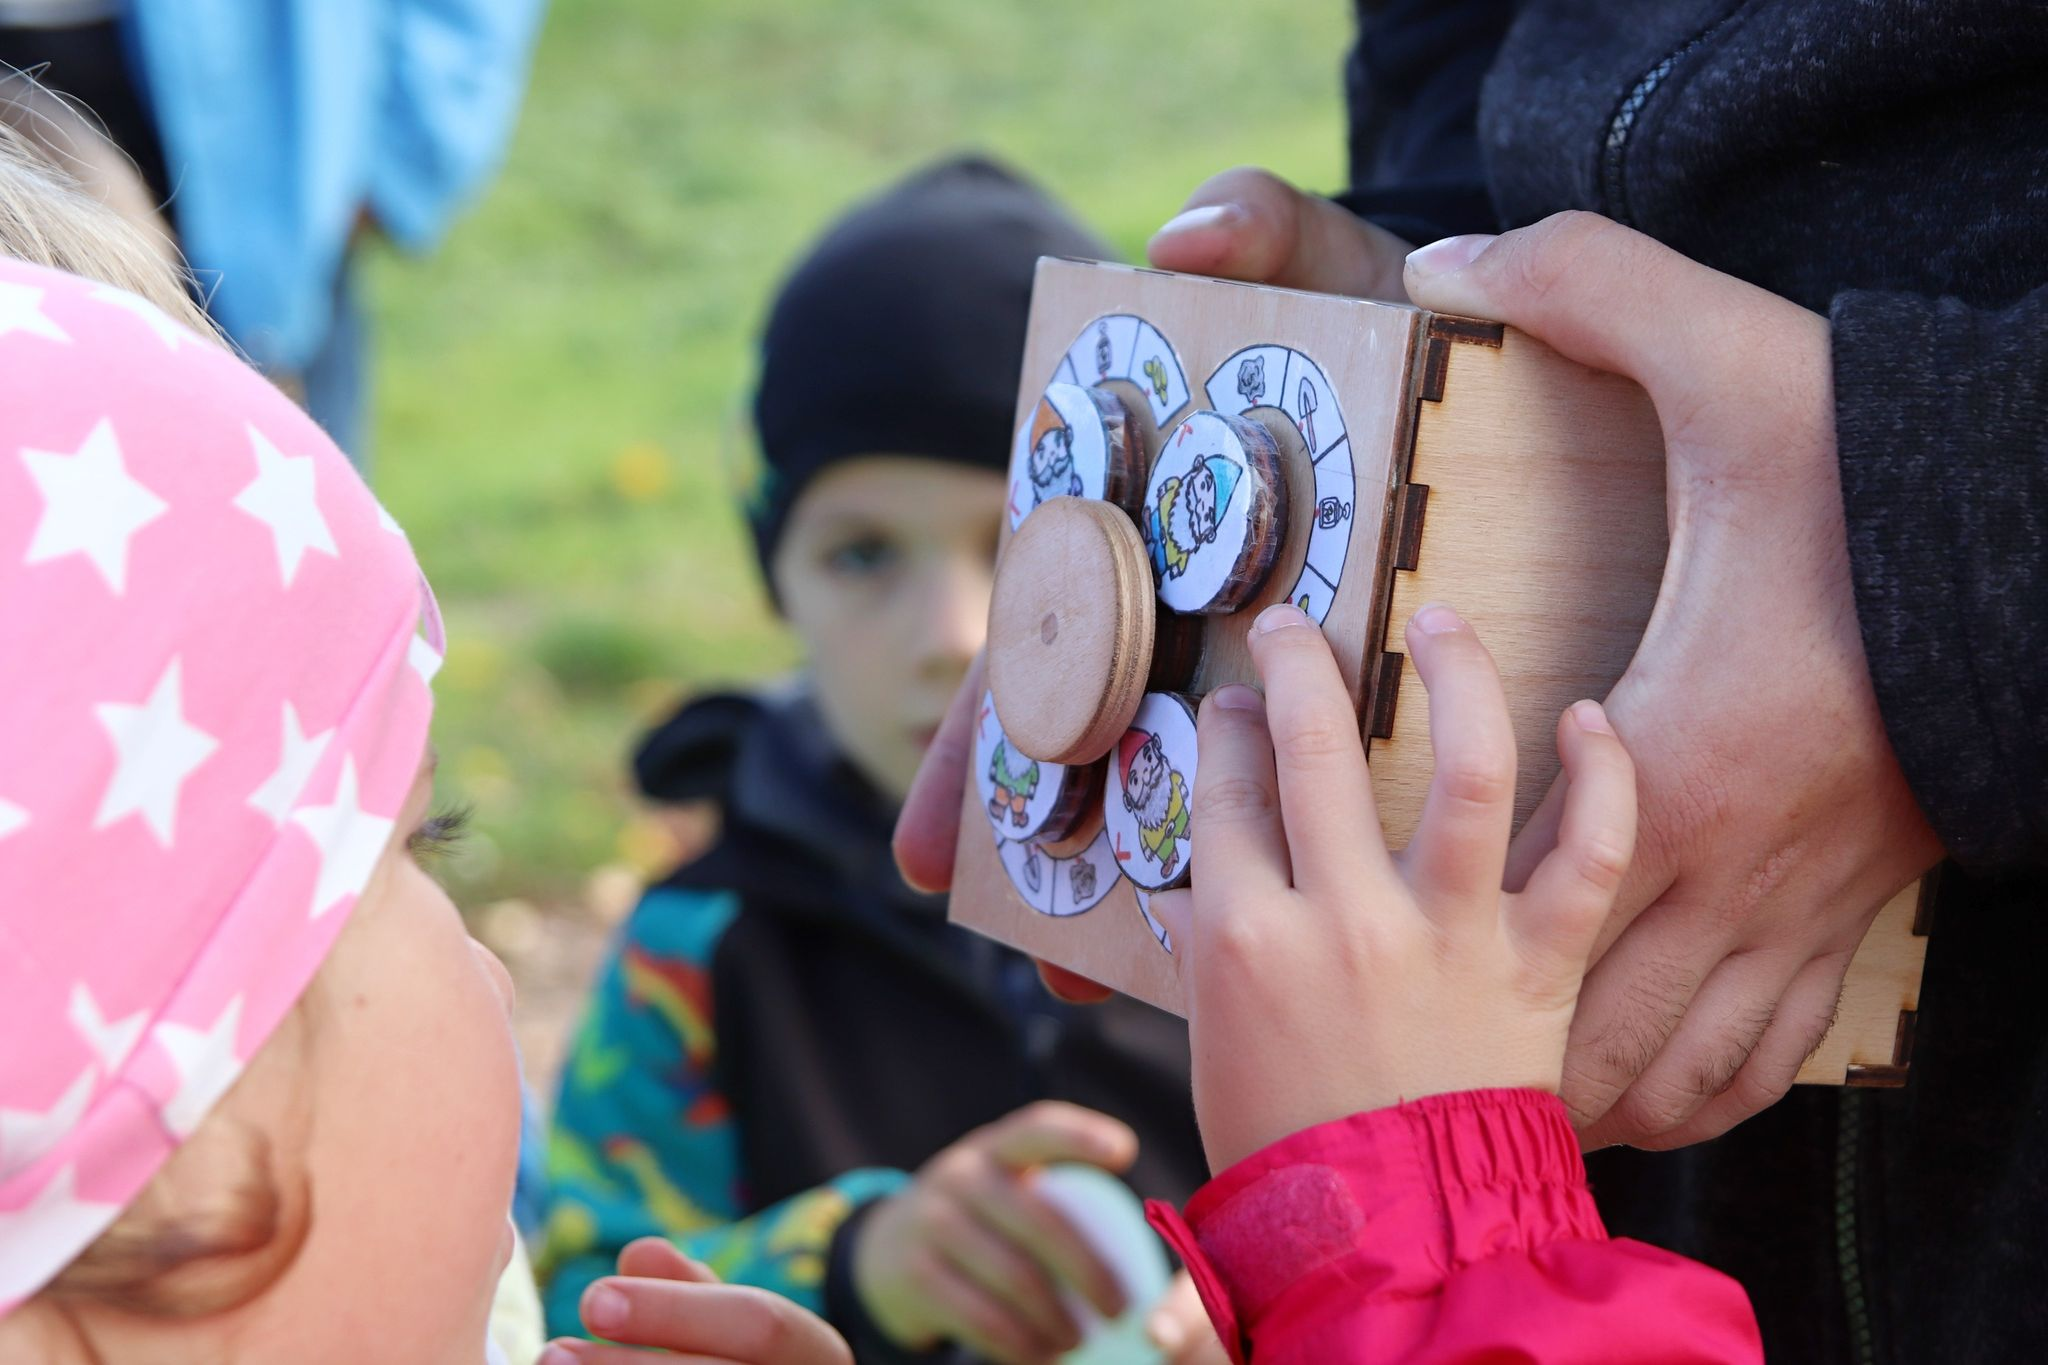
\includegraphics[width=\textwidth]{kapitoly/obrazky/M3/trpaslici.png}
    \caption{Trpasličí trezor}
    \label{fig:M3-trpaslici}
\end{figure}